% Resume of João Gabriel Salvador Paiva — Mobile profile (Flutter/Dart), English version
% Generic for mid-level Flutter Mobile Developer roles.
% Single-column layout, fully selectable text, no tables or text boxes (ATS-friendly).
\documentclass[10.5pt,a4paper]{article}

\usepackage[T1]{fontenc}
\usepackage[utf8]{inputenc}
\usepackage[english]{babel}
\usepackage{lmodern}
\usepackage[margin=1.5cm,top=1.2cm,bottom=1.2cm]{geometry}
\usepackage{graphicx}
\usepackage{enumitem}
\usepackage{titlesec}
\usepackage{xcolor}
\usepackage[hidelinks]{hyperref}
\usepackage{microtype}
\usepackage{needspace}

\definecolor{azul}{HTML}{14375A}

\hypersetup{
  pdftitle={Joao Gabriel Salvador Paiva - Mobile Developer Flutter},
  pdfauthor={Joao Gabriel Salvador Paiva},
  pdfsubject={Resume - Mobile Developer Flutter},
  pdfkeywords={Flutter, Dart, mobile, Android, iOS, App Store, Google Play, BLoC, state management,
  dependency injection, unit tests, widget tests, integration tests, REST API, FastAPI, Python, Git,
  Gitflow, CI/CD, GitHub Actions, Clean Code, SOLID, Scrum}
}

\pagestyle{empty}
\setlength{\parindent}{0pt}
\setlength{\emergencystretch}{2em}
\setlist[itemize]{leftmargin=3.6mm,itemsep=1pt,topsep=2pt,parsep=0pt,label=\textbullet}

\titleformat{\section}{\bfseries\large\color{azul}}{}{0em}{}[\vspace{-1.2ex}\rule{\linewidth}{0.6pt}]
\titlespacing{\section}{0pt}{2.2ex}{1.2ex}

\newcommand{\cargo}[4]{%
  \Needspace*{5\baselineskip}%
  \textbf{#1} \textnormal{---} #2 \hfill \textnormal{#3}\\
  \textit{\small #4}\vspace{0.4ex}
}

\begin{document}

%% ---------- Header ----------
\begin{minipage}[c]{0.78\textwidth}
\raggedright
{\LARGE\bfseries\color{azul} João Gabriel Salvador Paiva}\\[0.6ex]
{\large Mobile Developer --- Flutter \& Dart}\\[0.9ex]
\small
Campina Grande, Brazil (open to remote work)\\
\href{mailto:joaogabrielsalvadorpaiva@gmail.com}{joaogabrielsalvadorpaiva@gmail.com} $\cdot$ +55 (83) 98863-6734\\
\href{https://github.com/Ilusinusmate}{github.com/Ilusinusmate} $\cdot$
\href{https://www.linkedin.com/in/joao-gabriel-salvador-paiva-805283286}{linkedin.com/in/joao-gabriel-salvador-paiva} $\cdot$
\href{https://ilusinusmate.github.io/Ilusinusmate/}{ilusinusmate.github.io/Ilusinusmate}
\end{minipage}\hfill
\begin{minipage}[c]{0.2\textwidth}
\raggedleft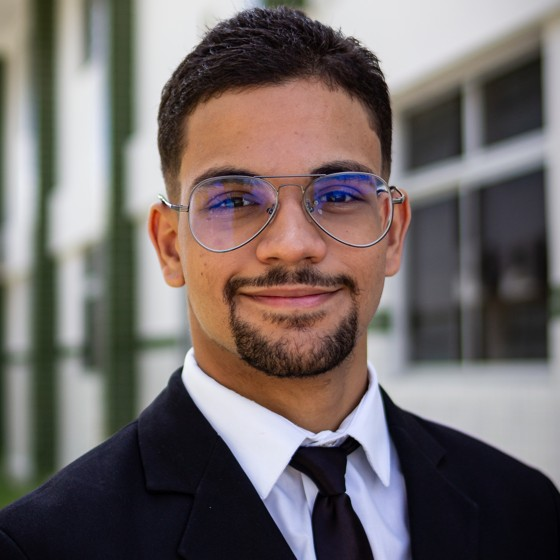
\includegraphics[width=2.7cm]{foto.jpg}
\end{minipage}

%% ---------- Summary ----------
\section*{Summary}
Mobile developer responsible for the \textbf{Central da Escola} application
(\textbf{Flutter/Dart}), with more than \textbf{50 thousand active users}; I have been its sole
developer since version 3 and lead the mobile development area. I cover the product's full cycle:
feature implementation, \textbf{testing}, \textbf{CI/CD}, \textbf{publication on Android and iOS
stores}, production monitoring and continuous evolution. I also develop the \textbf{backend}
supporting the app (\textbf{Python/FastAPI}, \textbf{REST APIs}, microservices and messaging),
enabling end-to-end integration between the application and its services. Computer Science
undergraduate at UFCG and ICT resident at VIRTUS-CC/UFCG.

%% ---------- Technical Skills ----------
\section*{Technical Skills}
\textbf{Mobile:} Flutter, Dart, Android, iOS, publication on Google Play and the App Store, state
management (BLoC), componentization, \textit{context isolation}, release cycle and production
monitoring\\
\textbf{Mobile quality:} unit tests, \textit{widget} tests and integration tests, code review,
Clean Code, SOLID, DRY, design patterns, layered architecture\\
\textbf{Integrations:} REST APIs, WebSocket, authentication, integrations with internal and
third-party systems\\
\textbf{Backend (complementary):} Python, FastAPI, Django, microservices, PostgreSQL, NoSQL, Redis,
RabbitMQ, MinIO\\
\textbf{Engineering:} Git (\textit{feature branches} and \textit{pull requests}), GitHub Actions,
CI/CD, Docker, AWS, logging and observability (OpenTelemetry, Grafana), technical documentation,
Scrum/Kanban

%% ---------- Professional Experience ----------
\section*{Professional Experience}

\cargo{Logon Informática}{Mobile \& Backend Developer}{Jan 2025 -- Present}{Software house for
education management, public administration and other sectors}
\begin{itemize}
  \item Sole developer of the \textit{Central da Escola} application since \textbf{version 3}, in
        \textbf{Flutter/Dart}, with more than \textbf{50 thousand active users} on Android and iOS.
  \item \textbf{Lead the mobile development area}: feature definition, prioritization, code review
        and team technical documentation.
  \item Conduct the \textbf{full release cycle}: development, testing, \textbf{CI/CD} and
        \textbf{publication on Google Play and the App Store}, with logging and production
        application monitoring.
  \item Develop the \textbf{Python/FastAPI microservices} consumed by the app, with \textbf{REST
        APIs}, asynchronous communication through \textbf{RabbitMQ} and object storage in
        \textbf{MinIO}.
  \item Act as a \textbf{liaison between teams} (product, backend and internal areas) for internal
        integrations and integrations with third-party systems.
  \item Published \textbf{pdfa-parser} on PyPI, an open-source PDF/A conversion and validation
        library used to support the company's products.
\end{itemize}

\cargo{Empório Sertanejo}{Full-stack Developer --- technical lead}{Dec 2023 -- Sep 2025}{Retail
franchise; proprietary ERP, POS and e-commerce SaaS}
\begin{itemize}
  \item \textbf{Led 3 developers} in building a SaaS that unified \textbf{ERP, POS and e-commerce},
        using \textbf{Django/Python}, \textbf{PostgreSQL} and \textbf{Docker}.
  \item Implemented \textbf{automated tests} (PyTest and mocks), \textbf{CI/CD with GitHub Actions}
        and \textbf{observability} (OpenTelemetry and Grafana) to investigate errors in staging and
        production.
  \item Conducted requirements gathering and direct negotiation with the client for more than
        2 years, delivering revenue-related features (loyalty program, coupons and notifications).
\end{itemize}

\cargo{VIRTUS-CC / Softex (UFCG)}{ICT Resident --- ISE group researcher}{Nov 2025 --
Present}{One-year software residency program: 240h of training + practical immersion}
\begin{itemize}
  \item Ranked \textbf{1st} in the selection process (96/100 in the titles evaluation and 100/100
        in the interview).
  \item Training in Software Engineering I and II, \textbf{agile methodologies}/Scrum, IoT,
        machine learning and design thinking, with projects in a \textbf{multidisciplinary squad}.
  \item Research in the \textbf{Intelligent Software Engineering} group on the use of LLMs in
        Software Engineering, with an article accepted at \textbf{XP 2026} (Springer LNBIP).
\end{itemize}

\cargo{Animalesko}{Backend Developer (volunteer)}{Apr 2024 -- Sep 2024}{Social startup supporting
stray animals}
\begin{itemize}
  \item Designed a \textbf{cross-platform} architecture (mobile and desktop over a single
        infrastructure), prioritizing low resource consumption, and documented technical decisions.
\end{itemize}

\cargo{IFPB (CNPq / LAPLIN)}{Scholarship researcher and Python instructor}{2023 -- 2024}{Natural
Language Analysis and Processing Laboratory}
\begin{itemize}
  \item Taught \textbf{Python} classes to approximately 60 students and led the student research
        group, with publications at national events.
\end{itemize}

%% ---------- Mobile Projects ----------
\section*{Mobile Projects}
\begin{itemize}
  \item \textbf{Central da Escola} (Logon) --- Flutter school app with \textbf{50 thousand+ active
        users}, published on Android and iOS, with its own supporting microservices.
  \item \textbf{TodoApp} --- Flutter app built as a deliberate exercise in \textbf{Clean Code},
        \textbf{SOLID}, componentization, \textit{context isolation} and \textbf{BLoC} as the state
        manager, running on Android and Linux Desktop:
        \href{https://github.com/Ilusinusmate/todoApp}{github.com/Ilusinusmate/todoApp}
  \item \textbf{ChatApp} --- Flutter mobile chat integrated with a custom FastAPI backend, exercising
        real-time communication and REST API consumption.
  \item \textbf{Corretor ONHB} --- solution for automatic correction of National History Olympiad
        exams, commissioned by IFPB teachers, in mobile (Flutter) and desktop (Electron) versions,
        used by more than 30 teams.
  \item \textbf{Scheduling app --- Clínica Dra. Daiane de Lima} --- scheduling, customer and
        inventory management, replacing a paper-based process; freelance project from problem
        definition to delivery.
\end{itemize}

%% ---------- Education ----------
\section*{Education}
\textbf{Bachelor of Computer Science} --- Federal University of Campina Grande (UFCG)
\hfill Jan 2025 -- 2030\\
\textbf{Integrated Technical Program} --- Federal Institute of Paraíba (IFPB)
\hfill Mar 2022 -- Dec 2024\\
\textbf{Additional training} --- Flutter Specialist and Python Backend Developer (DIO)

%% ---------- Publications and Awards ----------
\section*{Publications and Awards (selected)}
\begin{itemize}
  \item \textbf{8 scientific works} published on AI, LLMs and Software Engineering, including an
        article at \textbf{XP 2026} (Springer LNBIP, 2nd author) and articles at \textbf{WEI 2025}
        and \textbf{WICS 2024} (Brazilian Computer Society).
  \item \textbf{Best expanded abstract} in the Scientific and Technological Initiation --- ICT
        category at the \textbf{5th SIMPIF} (2023).
  \item \textbf{Champion of the Paraíba Informatics Olympiad} (2023), \textbf{gold} in the Advanced
        Junior category (2026) and finalist in the Brazilian Informatics Olympiad (2023).
\end{itemize}

\section*{Languages}
Portuguese (native) $\cdot$ English (advanced --- reading, writing and professional communication)
$\cdot$ Libras/Brazilian Sign Language (intermediate)

\end{document}
